\documentclass[10pt]{article}
\usepackage{adjustbox}
\usepackage{booktabs}
\usepackage{graphicx}
\usepackage{graphics}
%\usepackage{subcaption}
\usepackage{caption}
\usepackage{mathtools}
\usepackage{tikz,pgfplots}
\usepackage{subfig}
\usepackage{epsfig}
\usepackage{amsmath}
\usepackage{amssymb}
\usepackage[shortlabels]{enumitem}
\usetikzlibrary{angles,patterns,calc}
\usepackage{bbm}
\usepackage{float}
\usepackage{natbib}
\usepackage[sc]{mathpazo}
\usepackage[T1]{fontenc}
\usepackage{amsfonts}
\usepackage[onehalfspacing]{setspace}
\usepackage[margin=.75in, tmargin=0.71in, bmargin=0.71in]{geometry}
\usepackage{url}
\usepackage{appendix}
\usepackage{hyperref}
\usepackage{xcolor}
\usepackage{todonotes}
\usepackage{lscape}
\usepackage{comment}
\usepackage{amsthm}
\newcommand\der[2]{\frac{\partial{#1}}{\partial{#2}}}
\DeclareMathOperator*{\argmax}{arg\,max}
\DeclareMathOperator*{\argmin}{arg\,min}
\newtheorem{claim}{Claim}
\newtheorem{claimproof}{Proof of claim}[claim]

% stuff to put matlab code in 
\usepackage{listings}
\usepackage{color} %red, green, blue, yellow, cyan, magenta, black, white
\definecolor{mygreen}{RGB}{28,172,0} % color values Red, Green, Blue
\definecolor{mylilas}{RGB}{170,55,241}

% Shortcut greek
\def\a{\alpha}
\def\b{\beta}
\def\g{\gamma}
\def\D{\Delta}
\def\d{\delta}
\def\z{\zeta}
\def\k{\kappa}
\def\l{\lambda}
\def\n{\nu}
\def\r{\rho}
\def\s{\sigma}
\def\t{\tau}
\def\x{\xi}
\def\w{\omega}
\def\W{\Omega}

\usepackage[utf8]{inputenc}
\usepackage[english]{babel}
\usepackage{fancyhdr}
\fancypagestyle{firststyle}
{
\fancyhf{}
    \renewcommand{\headrulewidth}{0pt}
   \fancyfoot[C]{\footnotesize Page \thepage\ of \pageref{LastPage}}
}

\newcommand{\numpy}{{\tt numpy}}    % tt font for numpy

% Custom proof formatting: https://tex.stackexchange.com/questions/8089/changing-style-of-proof
\renewcommand\qedsymbol{$\blacksquare$}
\makeatletter
\renewenvironment{proof}[1][\proofname] {\par\pushQED{\qed}\normalfont\topsep6\p@\@plus6\p@\relax\trivlist\item[\hskip\labelsep\bfseries#1\@addpunct{.}]\ignorespaces}{\popQED\endtrivlist\@endpefalse}
\makeatother

\usepackage[autostyle, english = american]{csquotes}
\MakeOuterQuote{"}

\topmargin -.5in
\textheight 9in
\oddsidemargin -.25in
\evensidemargin -.25in
\textwidth 7in

\newcommand{\question}[1]{ \begin{center} \noindent\colorbox{gray!10}{
\parbox{0.8\textwidth}{\vspace{0.125in} #1 \vspace{0.125in} } } \end{center} }

\floatplacement{table}{H}
\floatplacement{figure}{H}

\pgfplotsset{compat=1.17}

\begin{document}

    \thispagestyle{firststyle}

    \title{Principal Component Regression as a Solution to Measurement Error Bias\thanks{The code for this paper can be found at \url{https://github.com/ijyliu/ECMA-31330-Project}.}} 
    \author{Isaac Liu, Nicol\'as Martorell \& Paul Opheim}
    \maketitle

    % code

    \lstset{language=Matlab,%
        %basicstyle=\color{red},
        breaklines=true,%
        morekeywords={matlab2tikz},
        keywordstyle=\color{blue},%
        morekeywords=[2]{1}, keywordstyle=[2]{\color{black}},
        identifierstyle=\color{black},%
        stringstyle=\color{mylilas},
        commentstyle=\color{mygreen},%
        showstringspaces=false,%without this there will be a symbol in the places where there is a space
        numbers=left,%
        numberstyle={\tiny \color{black}},% size of the numbers
        numbersep=9pt, % this defines how far the numbers are from the text
        emph=[1]{for,end,break},emphstyle=[1]\color{red}, %some words to emphasise
        %emph=[2]{word1,word2}, emphstyle=[2]{style},    
    }

    \begin{abstract}

        We examine the use of Principal Component Regression (PCR) as a solution to bias introduced by measurement error in auxilliary covariates included in a regression. We show its usefulness through econometric theory and then use Monte Carlo simulations to show how it provides benefits for different parameters and correlations between the true covariate and the variable of interest. We then compare its performance with the performance of other methods for mitigating measurement error-induced bias, and discuss the situations in which PCR is the ideal method for dealing with this issue. We then apply these methods to study the relationship between life expectancy and the level of government involvement in a country's healthcare system.
        
    \end{abstract}

    \newpage \clearpage

    \section*{Introduction}

        Many variables of interest in economics are not directly available as empirical data. Instead, economists often use other variables that are imperfect measurements of the true focus of their analysis. These available variables are known as \textit{proxies} or ``variables measured with error'', and, if they suffer from classical measurement error, are relevant for the model specification, and are correlated with the variable of interest, their use biases the coefficient of the variable of interest even if it does not suffer of measurement error. Traditionally, instrumental variables are used to get rid of measurement error induced bias.

        As an alternative method of dealing with this problem, we propose the use of Principal Component Analysis (PCA) over several variables measured with error. When there are multiple observed variables driven by a single ``true'' one, we propose to use PCA over these variables to extract the ``true'' variable. One may then use this extracted value in a standard OLS regression (often referred to as PCR or Principal Components Regression), thus providing a way to identify the parameter of interest that does not require the assumptions of instrumental variable analysis. The method also allows for more complex and possibly more optimal weightings of mismeasurements relative to simple averaging, and is less vulnerable to the curse of dimensionality relative to the inclusion of many covariates.

        This estimator ties into earlier literature considering the intersection of factor models and principal components analysis and measurement error and latent variables problems. Somewhat similarly to our methods, \cite{nagasawa_identication_2020} develops the use of a proxy variable to deal with unobserved heterogeneity in nuisance parameters and uses a partial effects method. Differing from most of scenarios considered, \cite{schennach_recent_2016} focuses on nonclassical measurement error and nonlinear cases and notes the usefulness of factor methods and some cases where they are of more use than instrumental variables. \cite{wegge_local_1996} considers a setting in which measurement error regression models are factor analysis models, with the correct regressors being the factors. Latent factors are uncorrelated with the errors. Focusing on measurement error in the main regressor, \cite{schofield_correcting_2015} combines solutions from structural equations modelling and item response theory to deal with misestimation. Finally, \cite{heckman_matching_2010} considers a situation similar to ours, except involving matching estimators. Without correction, matching estimators can be harmed by mismeasured conditioning variables. However, average treatment effects can be identified using factor proxies, and without need for normalization.

        In this paper, we present a theoretical framework and a Monte-Carlo analysis in order to show the properties and behavior of our estimator on large samples under standard assumptions. Additionally, we explore a basic empirical application of our method, by estimating the relationship between economic development on life expectancy at birth. Since there is no consensus on how to measure economic development, we take a sample of different variables that may measure economic development with error (GDP per capita, GNI per capita, Income per Employed Person, among others) over which we apply PCA to estimate coefficients. Our estimator generally behaves as expected in this empirical setting, though it is unclear whether it performs any better or worse than the direct inclusion of covariates, their averaging, or the instrumentation of mismeasured variables with each other.

    \section*{Theoretical framework}

        Consider a model where the outcome is denoted by $y_i$. This outcome depends on a variable of interest denoted by $t_i$ and a vector of covariates denoted by $X_i=(x_{i,1},x_{i,2},\dots x_{i,p})'$. Additionally, consider a vector of variables $X^*_i=(x^*_{i,1},x^*_{i,2},\dots x^*_{i,p})'$ that correspond to the covariates $X_i$ but observed with measurement error, where $x^*_{i,k}=x_{i,k}+\eta_{i,k}$ with $\eta_{i,k} \sim {iid}(0,\sigma^2_{\eta_k})$, $\operatorname{E}(x_{i,k}'\eta_{i,k})=0, \forall i$, $\operatorname{E}(x_{i,k}'\eta_{j,l})=0, \forall i\neq j$ and $k \neq l$, and $\operatorname{E}(\eta_{i,k}'\eta_{j,l})=0, \forall i\neq j$ and $k \neq l$. Therefore, each $x^*_{i,k}$ suffers classical measurement error. Note that $\operatorname{E}(x_{i,k})=\operatorname{E}(x^*_{i,k})=\mu_{x_k}$ and that $\operatorname{V}(x_{i,k})=\sigma^2_{x_k}$ while $\operatorname{V}(x^*_{i,k})=\sigma^2_{x_k}+\sigma^2_{\eta_k}\geq \sigma^2_{x_k}$.
        
    \subsection*{Data Generation Process}
        
        Assume that the outcome $y_i$ is determined by the following Data Generation Process (DGP):
        \begin{align}
            y_i = \gamma t_i + X_i'\beta + \epsilon_i
        \end{align}
        
        where $\g$ is the parameter of the variable of interest $t_i$, $\b=(\b_1,\b_2,\dots \b_p)'$ is the vector of the parameters of the covariates $X_i$ including a constant and $\epsilon_i \sim \operatorname{iid}(0,\sigma^2_\epsilon)$. Under this specification, the coefficients are such that:
        \begin{align} \label{true_coeffs}
            \left(\begin{array}{l}
        {\gamma} \\
        {\beta}
        \end{array}\right)=\left(\begin{array}{cc}
        {\sigma}^2_{t} & \Sigma_{tX} \\
        \Sigma_{Xt} & {\Sigma}_{X}
        \end{array}\right)^{-1}\left(\begin{array}{c}
        \Sigma_{yt} \\
        \Sigma_{yX}
        \end{array}\right)
        \end{align}
        
        Suppose that the econometrician has access to $t_i$ but, instead of $X_i$ she observes $X^*_i$. Then, she specifies the following linear model:
        \begin{align}
            y_i = \gamma^* t_i + {X^{*}_i}' \beta^* + \zeta_i
        \end{align}
        
        The coefficients would be such that:
        \begin{align} \label{mismeasured_coeffs}
            \left(\begin{array}{l}
        {\gamma}^* \\
        {\beta}^*
        \end{array}\right)
        & =\left(\begin{array}{cc}
        {\sigma}^2_{t} & \Sigma_{tX} \\
        \Sigma_{Xt} & {\Sigma}_{X}+{\Sigma}_{\eta}
        \end{array}\right)^{-1}\left(\begin{array}{cc}
        {\sigma}^2_{t} & \Sigma_{tX} \\
        \Sigma_{Xt} & {\Sigma}_{X}
        \end{array}\right)\left(\begin{array}{l}
        {\gamma} \\
        {\beta}
        \end{array}\right)
        \end{align}
        
        Without loss of generality, assume that the abovementioned DGP consists only of two variables as follows:
        \begin{align}
                    y_i = \gamma^* t_i +  \beta^*x_i* + \zeta_i
        \end{align}
        
        Then the coefficient of our variable of interest will be biased.
        \begin{claim}
        \label{claim:one}
        Under measurement error in the covariates, the coefficient is such that:
            \begin{align}
                \gamma^* = \gamma + \beta\frac{\operatorname{cov}(t,x)(\sigma^2_{x^*}-\sigma^2_x)}{\sigma_{t}^2\sigma_{x^*}^2-\operatorname{cov}({t,x})^2}
            \end{align}
        \end{claim}

        \begin{proof}
            See Theory Appendix.
        \end{proof}

       From Claim \ref{claim:one} it is clear that when $\operatorname{cov}(t,x)\neq 0$ and that $x$ is measured with error (i.e $\sigma_{x^*}^2>\sigma_x^2)$, the coefficient of our variable of interest is biased. If $t$ and $x$ are independent, then measurement error in $x^*$ does not cause any bias. If there is no measurement error in $x^*$, then $\sigma^2_{x^*}=\sigma^2_x$ and so we would not face any kind of bias, as one would expect.
        
        Claim \ref{claim:one} also allows us to know the direction of the bias. Given that we are facing measurement error in the covariate, $\sigma^2_{x^*}>\sigma^2_x$ which implies $\sigma^2_{x^*}-\sigma^2_x>0$. Also, it follows from the \textit{Cauchy-Schwarz} inequality that the denominator is also positive. Then, the direction of the bias will depend on the sign of $\beta$ and the covariance of $t$ and $x$, as Table \ref{bias_direction} illustrates.
        
        \begin{table}[H]
            \centering
            \caption{Direction of the Bias due to Measurement Error in the Covariate}
            \label{bias_direction}
            \begin{tabular}{|c|c|c|}\hline \hline
              & $\b>0$  & $\b<0$ \\ \hline
             $\operatorname{cov}(t,x)>0$ & upward-biased & downward-biased \\ \hline
             $\operatorname{cov}(t,x)<0$ & downward-biased & upward-biased \\ \hline
            \end{tabular} 
        \end{table}
        
    \subsection*{Principal Component Regression as a Bias Correction Method}
        
        The classical solution for the measurement-error induced bias in econometrics has been the usage of instrumental variables. Suppose we use as an instrument $Z_i$ another measure of $X_i$ so that
        \begin{align}
            Z_i=X_i+\omega_i
        \end{align}
        where $\operatorname{E}(\omega_i)=0$, $\operatorname{Cov}(\epsilon_i,\omega_i)=0$ and that $\omega_i$ brings new information so that $\operatorname{Cov}(\eta_i,\omega_i)=0$.  Under these conditions, $Z_i$ is a valid instrument.

        \begin{claim}
        Suppose $ Z_i=X_i+\omega_i$. If $\operatorname{E}(\omega_i)=0$, $\operatorname{Cov}(\epsilon_i,\omega_i)=0$ and $\operatorname{Cov}(\eta_i,\omega_i)=0$. Then
        \begin{align}
        \operatorname{E}(Z_i\zeta_i)=0 \ \text{and} \  \operatorname{E}(Z_iX_i)\neq0
        \end{align}
        And so $\gamma$ can be identified through IV regression.
        \end{claim}

        \begin{proof}
        See Theory Appendix.
        \end{proof}
        
        Alternatively, we propose an alternative bias-correction method when there are several mismeasured variables for each covariate; that is when we have more than one $x_{i,k}^*$ for every $x_{i,k}$. Given that in all the mismeasured variables the underlying value is the real value, one could think of extracting the underlying true $x_{i,k}$ through a linear combination of the different $x_{i,k}^*$. Then, we could treat all the $x_{i,k}^*$ as variables that share components as follows:

        \begin{align} \label{variance_max}
           h_{j}=\underset{h^{\prime} h=1, h^{\prime} h_{1}=0, \ldots, h^{\prime} h_{j-1}=0}{\operatorname{argmax}} \operatorname{var}\left[h^{\prime} X^*_k\right]  
        \end{align}
        
        where $h_j$ is the eigenvector of $\Sigma$ associated with the $j^{t h}$ ordered eigenvalue $\lambda_{j}$ of $\Sigma_{X^*_k}$, and the principal components of $X^*_k$ are $U_{j}=h_{j}^{\prime} X^*_k$, where $h_{j}$ is the eigenvector of $\Sigma$ associated with the $j^{t h}$ ordered eigenvalue $\lambda_{j}$ of $\Sigma$. Then, we could then retrieve the vector of true variables $X_i$.

        \begin{claim} \label{linear_combo}
            \begin{align}
                X_i=HX^*_i
            \end{align}
        where $H$ is a matrix composed of the $h_k$ vectors of eigenvalues of $x_{i,k}$, $\forall i,k$.
        \end{claim}

        \begin{proof}
            See Theory Appendix.
        \end{proof}
 
        Our new linear model then would be:
        \begin{align} \label{eigen_lc}
            y_i = \gamma^{PCR} t_i + H{X^*_i}'\beta^{PCR} + \epsilon_i
        \end{align}
        
        where $\gamma$ is identified.

        \begin{claim}
        Consider equation (\ref{eigen_lc}). Then
            \begin{align}
                {\gamma}^{PCR} = \gamma
            \end{align}
        \end{claim}

        \begin{proof}
            See Theory Appendix.
        \end{proof}
        
        Note that according to Claim \ref{linear_combo}, the true variable $x_{i,k}$ is a linear combination of the mismeasured variables that the researcher may have, where the weights are such that equation $(\ref{variance_max})$ is satisfied. This allows us to think about other linear combinations that could be used as a bias-correction method which need not satisfy (\ref{variance_max}). 
        
        In particular, take the case in which $h_k='(\frac{1}{n},\frac{1}{n},\dots,\frac{1}{n})$, where $h_k$ is a row vector of dimension $(1\times J)$, and $J$ is the number of mismeasured variables for $x_{i,k}$. Then, Claim \ref{linear_combo} will be
        \begin{align}
            \Tilde{x_{i,k}}&=\left(\begin{array}{cccc}
            \frac{1}{n} & \frac{1}{n} & \dots &\frac{1}{n} 
            \end{array}\right)\left(\begin{array}{l}
            x^*_{i,1} \\
            x^*_{i,2} \\
            \vdots \\
            x^*_{i,J} 
            \end{array}\right)\\
            &=\frac{1}{n}\sum_{j=1}^J x^*_{i,j}
        \end{align}
        
        That is, the average of the mismeasured variables for $x_{i,k}$ is a feasible linear combination that may correct for the mismeasurement bias problem.

    \section*{Properties of the Estimator: Monte Carlo Simulations}

        We complement our theoretical analysis by using Monte Carlo Simulation to analyze the effects of using Principal Components Regression as a method of bias correction. For these simulations, we assume that the true DGP for the data is:

        $$y_i = \beta_1 x_i + \beta_2 z_i + u_i$$

        where $x_i$ and $z_i$ are single variables drawn from $\mathcal{N}(\begin{bmatrix} 0\\ 0 \end{bmatrix}, \begin{bmatrix} 1 & \rho\\ \rho & 1\end{bmatrix})$ and where $\rho$ is the covariance between our main variable of interest $x_i$ and the covariate $z_i$. The $u_i$ is drawn from a white noise distribution ($\mathcal{N}(0,1)$) that is uncorrelated with both $x_i$ and $z_i$. We then assume (as with the theoretical analysis) that $z_i$ is not directly observable and instead the researchers only have access to $p$ measurements $z_{i,j}^*$ where $z_{i,j}^* = z_i + \eta_j$, where $\eta_j$ is drawn from a white noise distribution $\mathcal{N}(\mathbf{0},\Sigma)$, where $\mathbf{0}$ is a p-vector, and where $\Sigma$ is the $p$ by $p$ identity matrix.

        In our simulations, we assume default values of $\rho = 0.5$, $\beta_1 = \beta_2 = 1$, and $p=5$. These values were chosen to best match the empirical application presented later in this paper. We then vary each factor while holding the others fixed, and perform 1,000 simulations of the DGP followed by an OLS regression on either the PCA value from the $p$ measurements of the true $z_i$, or on a single one of the measurements of $z_i$. For each simulation, we generate 3,000 observations of $y_i,x_i$, etc. The first two rows of each panel in Table \ref{sim_rho_3000_no_exp} show the results for different values of $\rho$.

        \begin{table}[!htbp] \centering
            \caption{Average Coefficients for Values of $\rho$ ($N=3,000$, No Exponential Transformation) \label{sim_rho_3000_no_exp}}
            \scalebox{0.75}{
            \begin{tabular}{@{\extracolsep{5pt}}lccccc}
        \\[-1.8ex]\hline
        \hline \\[-1.8ex]
        & \multicolumn{5}{c}{$\rho$ \textit{ Value}} \
        \cr \
        \\[-1.8ex] & -0.9 & -0.5 & 0 & 0.5 & 0.9 \\
        \hline \\[-1.8ex]
        & \multicolumn{5}{c}{\textit{Coefficient on Main Variable}} \\
        PCA &   0.538 &   0.895 &     1.0 &   1.106 &   1.462 \\
                        & (0.034) & (0.022) & (0.019) & (0.022) & (0.034) \\
     Single Measurement &   0.244 &   0.714 &   0.999 &   1.286 &   1.756 \\
                        & (0.025) & (0.023) & (0.022) & (0.022) & (0.026) \\
       All Measurements &   0.538 &   0.895 &     1.0 &   1.106 &   1.462 \\
                        & (0.033) & (0.023) & (0.019) & (0.022) & (0.034) \\
Average of Measurements &   0.538 &   0.895 &     1.0 &   1.106 &   1.462 \\
                        & (0.034) & (0.022) & (0.019) & (0.022) & (0.034) \\
  Instrumental Variable &   0.994 &   0.999 &     1.0 &     1.0 &   1.002 \\
                        & (0.116) & (0.048) & (0.037) & (0.039) & (0.115) \\
            & \multicolumn{5}{c}{\textit{Mean Absolute Percentage Error}} \\
            PC 1 & 46.2\% & 10.5\% & 1.5\% & 10.6\% & 46.2\% \\
     Single Measurement & 75.6\% & 28.6\% & 1.7\% & 28.6\% & 75.6\% \\
       All Measurements & 46.2\% & 10.5\% & 1.5\% & 10.6\% & 46.2\% \\
Average of Measurements & 46.2\% & 10.5\% & 1.5\% & 10.6\% & 46.2\% \\
  Instrumental Variable &  8.6\% &  3.3\% & 2.7\% &  3.0\% &  8.7\% \\ \\[-4mm]
            \hline \\[-1.8ex]
            Simulations & 1,000 & 1,000 & 1,000 & 1,000 & 1,000\\
        \hline
        \hline \\[-1.8ex]
        \end{tabular}}
        \end{table}

        We first note that when $\rho = 0.5$ or $0.9$ then the coefficient on the variable of interest is artificially inflated when we use a single mismeasurement as a covariate (on average, for $\rho = 0.5$, it is roughly 1.29 instead of the true value of 1). Conversely, when $\rho = -0.5$ or $-0.9$ then the coefficient is artificially deflated. Using the PCA value as the covariate reduces this bias for both directions, and brings the main coefficient closer to its true value of 1.0. These results are consistent with our theoretical section, where we argued that a positive covariance between the main variable and the true covariate will lead to an inflation on the main coefficient, while a negative covariance will lead to a deflation of the coefficient. Separately, there is no bias when $\rho = 0$, as predicted. Since there no bias to correct, we do not see gains from using the PCA covariate method for that particular $\rho$ value. These simulation results suggest that using PCR is more effective than a single mismeasured covariate, although there are no gains to using it when the covariance between the covariate and the main variable of interest is close to $0$. 

        However, the performance advantages that we see from using PCR could be driven by the benefit of having multiple measurements of our true covariate of interest, as opposed to any special advantages from PCR specifically. We test this question by comparing the estimated $\beta_1$ in our PCR regressions with the estimated $\beta_1$ when we include all $p$ measurements as separate covariates in the regression, and the $\beta_1$ obtained when the covariate is the mean of all $p$ measurements of the true covariate. We also show the results for an instrumental variables regression where we use other measurements of the true covariate as an instrument for a single measurement of the covariate. The results from these regressions for different values of $\rho$ are shown in the bottom three rows of each panel of Table \ref{sim_rho_3000_no_exp}.

        As one can see from these results, there does not seem to be a noticeable difference between using PCR, all measurements, or the average of measurements. However, the instrumental variable regression performs far better than these other methods, correcting for almost all bias and moving the estimated coefficient value close to 1 (although with noticeably larger standard errors than the other methods). Thus, our simulations suggest that, in this framework, there are major benefits to having multiple measurements of a latent covariate of interest. However, PCR does not noticeably improve on two other ways of incorporating these other measurements (taking their average or including all measurements as separate covariates) and performs much worse than using instrumental variables regression with these additional measurements.

        We then varied different aspects of this framework in order to better understand the conditions under which PCR performed especially well relative to the other possible methods for including multiple measurements of the same covariate. In this exploration, we discovered that when the ratio of $\frac{N}{p}$ is especially low (there are many measurements relative to the number of observations) then PCA starts to perform better than the instrumental variables method and the method where all measurements are included as separate covariates. We can thus see that PCR does reasonably well under the conditions known as "The Curse of Dimensionality".

        Additionally, we wanted to see how the different methods performed in a situation where the measurements of the true covariate are on different scales from one another.\footnote{This is often the case; for example, one could measure income inequality through a Gini coefficient and the percent of income that goes to the top 1\% of income-earners, but these variables are on totally different scales from each other.} To do this, we transform half of the covariate measurements by taking the $z_{i,j}^*$ value from before and transforming it, creating a new $z_{i,j}'$ value such that $z_{i,j}' = e^{z_{i,j}^*}$. We found that PCR tends to outperform taking the average of all covariate measurements under this multiple-scale measurement error framework. 
        
        We can see the effect of both a low $\frac{N}{p}$ ratio and transformed measurement errors in Table \ref{sim_p_pca_ideal}. The simulation appendix contains other useful charts for understanding the relative performance of PCR and these other methods.

        \begin{table}[!htbp] \centering
            \caption{Average Coefficients for Values of $p$ ($N=100$, Exponential Transformation) \label{sim_p_pca_ideal}}
            \scalebox{0.75}{
            \begin{tabular}{@{\extracolsep{5pt}}lccccc}
        \\[-1.8ex]\hline
        \hline \\[-1.8ex]
        & \multicolumn{5}{c}{$p$ \textit{ Value}} \
        \cr \
        \\[-1.8ex] & 5 & 20 & 50 & 100 & 500 \\
        \hline \\[-1.8ex]
        & \multicolumn{5}{c}{\textit{Coefficient on Main Variable}} \\
        PCA &   1.187 &   1.081 &    1.05 &   1.049 &   1.038 \\
                        & (0.137) & (0.127) & (0.122) & (0.123) & (0.118) \\
     Single Measurement &   1.286 &   1.289 &   1.284 &   1.291 &   1.282 \\
                        & (0.136) & (0.134) & (0.128) & (0.132) & (0.131) \\
       All Measurements &   1.162 &   1.056 &   1.019 &   0.971 &   0.098 \\
                        & (0.135) & (0.136) & (0.168) & (1.055) & (0.025) \\
Average of Measurements &   1.279 &   1.194 &   1.157 &    1.15 &   1.139 \\
                        & (0.147) & (0.141) & (0.137) & (0.138) & (0.132) \\
  Instrumental Variable &   1.011 &   1.103 &     1.2 &   1.291 &   1.282 \\
                        & (0.213) & (0.156) & (0.133) & (0.132) & (0.131) \\
        & \multicolumn{5}{c}{\textit{Mean Absolute Percentage Error}} \\
            PC 1 & 19.9\% & 12.0\% & 10.6\% & 10.5\% &  9.9\% \\
     Single Measurement & 28.8\% & 29.1\% & 28.5\% & 29.3\% & 28.4\% \\
       All Measurements & 17.8\% & 11.8\% & 13.4\% & 68.8\% & 90.2\% \\
Average of Measurements & 28.3\% & 20.4\% & 17.4\% & 16.8\% & 15.8\% \\
  Instrumental Variable & 16.4\% & 15.0\% & 20.8\% & 29.3\% & 28.4\% \\ \\[-4mm]
            \hline \\[-1.8ex]
            Simulations & 1,000 & 1,000 & 1,000 & 1,000 & 1,000\\
        \hline
        \hline \\[-1.8ex]
        \end{tabular}}
        \end{table}

        In Table \ref{sim_p_pca_ideal}, PCR outperforms the single measurement method and average method across all values of $p$. Additionally, we can note that when $N=100$ and $p=5$, PCR performs worse than IV and the inclusion of all measurements, but as $p$ increases it outperforms them, at least in terms of Mean Absolute Percentage Error. 

        It is worth noting that in a real-life situation where there were 500 measurements of a single covariate, a researcher could choose to disregard most measurements if it would be expected that adding them to their model reduced performance (as seems to be the case with IV when $p>20$ here). The usage of IV could be tailored to avoid the $p=50,100,$ and $500$ situations suggested by these charts. However, it is worth noting that, as measured by MAPE, PCR's performance when $p=500$ ($10\%$) is superior to that of IV when $p=5$ or $10$ ($16\%$ and $15\%$ respectively), although it displays more bias (average distance from the true value of $1$). In this scenario PCR is a valid option to reduce variance (captured by the MAPE) at the cost of this bias.

        Overall, these simulations tell us that PCR helps to reduce measurement error-induced bias in OLS regression with a latent covariate relative to including only a single measurement of that covariate. Additionally, within the framework most similar to our empirical application, it seems to perform in line with taking the average of those covariate measurements and using each measurement as a separate covariate in the regression, but worse than using an IV technique. However, there are circumstances where PCR is the best-performing technique of all the ones studied in this paper. This suggests that using PCR as a method for reducing measurement error-induced bias in the coefficient on the variable of interest can occasionally be helpful.

    \section*{Application: Government Share of Healthcare Spending and Life Expectancy}

        We now examine the usage of the principal components estimator in an empirical setting with measurement error. One interesting question in public economics and public health is the study of the relationship between publicly and privately funded healthcare systems and outcomes such as life expectancy. To measure the public or private nature of a healthcare system we use the continuous variable of the government's share of total health expenditure in a given country and year.

        Some previous work has covered this relationship. Considering that this topic has been studied in "relatively few papers," \cite{linden_life_2017} focus on the relationship between life expectancy at birth and public and private health expenditures for 34 OECD countries from 1970-2012 and find that both public and private health spending are important to life expectancy and are associated with each other. \cite{or_determinants_2000} predicts premature death in 21 OECD countries from 1970-1992, considering the public share of health expenditure, environmental factors, and GDP. He finds that a larger share of public spending is associated with lower rates of premature mortality for both males and females, and that controlling for GDP is important; it is also associated with less premature mortality. \cite{or_determinants_2000} also demonstrates the importance of our methods of reducing the number of covariates considered, as it includes many economic variables and fixed effects but examines only several hundred observations; the estimators used may be subject to an significant amount of variance.

        In this regression it is important to account for the role of a country's level of economic development. There is an extensive literature documenting the relationship between economic development and life expectancy. \cite{ling_testing_2017} finds that economic growth is associated with increased life expectancy in Malaysia, while considering the reverse causal direction \cite{acemoglu_disease_2007} finds improvements in life expectancy lead to little or no growth. Somewhat less obvious is the linkage between government provision of healthcare and development. In general, public goods provision and government spending, including in fields such as healthcare, has been linked to prosperity; low income countries may remain in such a state due to inefficient governments and inferior institutions \citep{wu_impact_2010}.

        However, economic development is liable to be measured with error. GDP measurements usually rely on company surveys, and the methodology within a country and for comparisons between countries through exchange rates or PPP adjustments may vary \citep{grishin_main_2019}. Other sources of error include the presence of the informal economy and non-monetary but productive work, the challenge of accurately measuring the value of digital services which often do not have visible prices, and government incentives to manipulate official statistics about growth \citep{charmes_informal_2012,ahmad_can_2017,nakamura_are_2016}.\footnote{Due to differences in statistical capacity and the larger relative size of the informal economy, it is possible that mismeasurement of economic development is particularly severe in developing countries. On the other hand, the presence of the digital economy may mean mismeasurement is larger in developed nations. This would constitute the presence of non-classical measurement error, but we only consider classical measurement error in this paper. It is also possible that the interaction of many forms of measurement produces error which is closer to classical assumptions.} Hence, this setup, with a covariate in regression subject to measurement error, fits the situation described in the theory and simulations in the previous sections.\footnote{It seems less likely that our variable of interest, the government's share of health spending, is measured with error. One would think most governments capable of monitoring their own spending better than economic activity in general. Furthermore, for this variable there would seem to be less governmental incentive to manipulate the statistic relative to GDP or other items.} In this case, we aim to to reduce possible bias in the coefficient of the government's share of health spending by making appropriate use of multiple measures of economic development.

        Our data on all measures comes from the World Bank \citep{the_world_bank_indicators_2021}. We remove country-years with missing values for any of the variables summarized in Table \ref{Sum_Stats} and standardize the economic covariates in the 5 uppermost rows by subtracting the mean and dividing by the standard deviation (in order to enable interpretable principal component analysis).

        \begin{table}
\centering
\caption{Summary Statistics}
\label{Sum_Stats}
\scalebox{0.75}{\begin{tabular}{lcccccc}
\toprule
                                    Variable &   Obs &      Mean &        SD &      Min &       Med &        Max \\
\midrule
GDP Per Capita PPP (Current International \$) & 3,143 & 16,443.76 & 19,173.04 & 435.08 & 9,331.99 & 141,634.96 \\
GDP Per Capita (Current USD) & 3,143 & 11,764 & 17,582.7 & 111.93 & 4,018.95 & 118,823.65 \\
GNP Per Capita PPP (Current International \$) & 3,143 & 15,980.12 & 18,478.14 & 410 & 9,080 & 132,440 \\
GNP Per Capita (Current USD) & 3,143 & 11,247.65 & 16,583.07 & 110 & 3,800 & 104,560 \\
ILO GDP Per Person Employed & 3,143 & 41,782.32 & 39,743.08 & 1,371.24 & 29,220.02 & 266,103.71 \\
Life Expectancy at Birth (All Population) & 3,143 & 69.55 & 9.26 & 39.44 & 71.78 & 84.21 \\
Government Share of Health Expenditure & 3,143 & 49.62 & 21.73 & 4.06 & 50.27 & 95.14 \\
\bottomrule
\end{tabular}}
\end{table}


        In Table \ref{main_regs} we apply our main set of estimators. The PCA estimator is found in column (1). In column (2), we instead control for just a single measurement of GDP per capita (PPP). In column (3) we directly include the full set of economic covariates (measurements) listed in the 5 uppermost rows of Table \ref{Sum_Stats}. In column (4), we use the mean of these mismeasured covariates, and in column (5) we perform instrumental variables regression using all the other economic indicators as an instrument for GDP per capita (PPP).

        \begin{table}[!htbp] \centering
  \caption{Regressions of Life Expectancy on Government Share of Health Spending \label{main_regs}}
\begin{tabular}{@{\extracolsep{5pt}}lccccc}
\\[-1.8ex]\hline
\hline \\[-1.8ex]
& \multicolumn{5}{c}{\textit{Life Expectancy at Birth (Years)}} \
\cr \
\\[-1.8ex] & (1) & (2) & (3) & (4) & (5) \\
\hline \\[-1.8ex]
 Govt. Share of Health Exp. & 0.596$^{***}$ & 0.404$^{***}$ & 0.342$^{***}$ & 0.358$^{***}$ & 0.358$^{***}$ \\
  & (0.019) & (0.020) & (0.019) & (0.019) & (0.019) \\
 Covariates & None & GDP PC PPP & Econ Indicators & Mean & PC 1 \\
\hline \\[-1.8ex]
 Observations & 1,799 & 1,799 & 1,799 & 1,799 & 1,799 \\
 $R^2$ & 0.355 & 0.464 & 0.553 & 0.512 & 0.511 \\
 Adjusted $R^2$ & 0.355 & 0.464 & 0.551 & 0.511 & 0.511 \\
 Residual Std. Error & 0.804 & 0.733 & 0.670 & 0.699 & 0.700  \\
 F Statistic & 989.324$^{***}$  & 778.290$^{***}$  & 369.354$^{***}$  & 942.234$^{***}$  & 939.771$^{***}$  \\
\hline
\hline \\[-1.8ex]
\textit{Note:} & \multicolumn{5}{r}{$^{*}$p$<$0.1; $^{**}$p$<$0.05; $^{***}$p$<$0.01} \\
\end{tabular}
\end{table}

        The PCA estimator indicates that a one percentage point increase in the government share of health expenditure is linked to a increase in life expectancy of 0.18 years. Notably, the results generally demonstrate that the methods using multiple measures of the covariates produce different coefficients for government health share, relative to the use of a single mismeasurement. The principal components estimator, the usage of many economic indicators directly, and their mean each produce far smaller coefficients. The IV estimator produces a slightly smaller coefficient.

        Moreover, these different coefficients behave in a manner similar to that predicted by our theoretical development and simulations. In Table \ref{sim_rho_3000_no_exp}, we saw the impact of variation in $\rho$, the correlation between measurements for a values of $p = 5$ and $\beta_1, \beta_2 = 1$ for 3,000 observations. In the empirical setting it is difficult to tell what is a reasonable value of $\beta$. Nevertheless, we see that for a positive $\rho$ value between 0 and 1 (as is likely to be the case in light the correlation between GDP and the government share of health spending and overall public goods), the coefficient obtained from using a single measurement is inflated relative to that from PCA, and presumably other methods combining multiple measures as in columns (3), (4), and (5) of Table \ref{main_regs}.

        % Compare iv performance

        Results using univariate OLS (with no covariates), country and year fixed effects models (with country clustered standard errors), and more principal components are in Table \ref{additional_regs}. Univariate OLS produces a large and inflated coefficient. Fixed effects coefficients greatly reduce the magnitude of any potential causal effects and are insignificant. The results in column (4) also show a reduction in the inflation of coefficients relative to column (2) of Table \ref{main_regs}, as the inclusion of more principal components produces a small coefficient very similar to that obtained with just a single component. \footnote{This is likely due to the high explanatory power of just the first principal component, as is clear in Appendix Figure \ref{Econ_Share_Explained}.}

        \begin{table}[!htbp] \centering
  \caption{Additional Regressions \label{additional_regs}}
\begin{tabular}{@{\extracolsep{5pt}}lcccc}
\\[-1.8ex]\hline
\hline \\[-1.8ex]
& \multicolumn{4}{c}{\textit{Life Expectancy at Birth (Years)}} \
\cr \
\\[-1.8ex] & (1) & (2) & (3) & (4) \\
\hline \\[-1.8ex]
 Govt. Share of Health Exp. & -0.004$^{}$ & -0.006$^{}$ & 0.321$^{***}$ & 0.335$^{***}$ \\
  & (0.022) & (0.022) & (0.014) & (0.014) \\
 Covariates & None & PC 1 & PC 1-2 & GDP PC (IV) \\
 Fixed Effects & Yes & Yes & No & No \\
\hline \\[-1.8ex]
 Observations & 4,066 & 4,066 & 4,066 & 4,066 \\
 $R^2$ & 0.974 & 0.974 & 0.453 & 0.399 \\
 Adjusted $R^2$ & 0.972 & 0.972 & 0.453 & 0.399 \\
 Residual Std. Error & 0.166 & 0.167 & 0.740 & 0.775  \\
 F Statistic & 264.787$^{***}$  & 140.640$^{***}$  & 1123.110$^{***}$  & nan$^{***}$  \\
\hline
\hline \\[-1.8ex]
\textit{Note:} & \multicolumn{4}{r}{$^{*}$p$<$0.1; $^{**}$p$<$0.05; $^{***}$p$<$0.01} \\
\end{tabular}
\end{table}

    \section*{Conclusion}
        
        In this paper, we have explored the usefulness of using Principal Component Regression (PCR) as a method of mitigating the bias on the coefficient for the main variable of interest that is induced by measurement error in an auxiliary covariate. Using theory and Monte Carlo simulations we have shown how this technique improves upon using a single measurement of the true covariate, and we have shown how its performance compares to that of some other methods for mitigating this bias. We then applied this technique to an empirical question (the relationship between the government share of health expenditure and life expectancy).

        Other solutions to measurement error meriting further exploration include the usage of general factor models, which could also involve the exploitation of the panel structure of relevant data. Measurements within time periods or units may provide information about the true value of variables. There are also likely other ways to summarize and control the dimension of the information presented by multiple measurements. Another option could be the usage of dimensionality-reduction techniques within an instrumental variables regression.

    \clearpage \newpage

    \bibliographystyle{aea}
    \bibliography{PCR_ME_Refs}

    \clearpage \newpage

    \appendix

	\section*{Theory Appendix}
	\subsection*{Short Proofs}

        \setcounter{claim}{0}
        \setcounter{claimproof}{0}

            \begin{claim} \label{claim_one_with_proof}
            Under measurement error in the covariates, the coefficient is such that:
            \begin{align*}
                    \gamma^* = \gamma + \beta\frac{\operatorname{cov}(t,x)(\sigma^2_{x^*}-\sigma^2_x)}{\sigma_{t}^2\sigma_{x^*}^2-\operatorname{cov}({t,x})^2}
                \end{align*}
            \end{claim}
            
        \begin{proof}

        Equations $(\ref{true_coeffs})$ and $(\ref{mismeasured_coeffs})$ will be such that
        \begin{align*}
                \left(\begin{array}{l}
            {\gamma}^* \\
            {\beta}^*
            \end{array}\right)&=\left(\begin{array}{cc}
            {\sigma}^2_{t} & \operatorname{cov}({t,x^*}) \\
            \operatorname{cov}({x^*,t}) & {\sigma}_{x^*}^2
            \end{array}\right)^{-1}\left(\begin{array}{c}
            \operatorname{cov}{(y,t)} \\
            \operatorname{cov}{(y,x^*)}
            \end{array}\right) \\
        \end{align*}
                
        \end{proof}	
        

        \begin{claim}
        Suppose $ Z_i=X_i+\omega_i$. If $\operatorname{E}(\omega_i)=0$, $\operatorname{Cov}(\epsilon_i,\omega_i)=0$ and $\operatorname{Cov}(\eta_i,\omega_i)=0$. Then
        \begin{align*}
        \operatorname{E}(Z_i\zeta_i)=0 \ \text{and} \  \operatorname{E}(Z_iX_i)\neq0
        \end{align*}
        And so $\gamma$ can be identified through IV regression.
        \end{claim}
        \begin{proof}

        Suppose an instrument $Z_i$ that satisfies the relevance condition $\operatorname{E}(Z_i'X_i)\neq 0$ and $\operatorname{E}(Z_i't_i)\neq 0$, and also the exclusion restriction $\operatorname{E}(Z_i'\epsilon_i)=\operatorname{E}(Z_i'\zeta_i)=\operatorname{E}(Z_i'\eta_{i,k})=0$, for all $i$ and $k$. Then premultiplying by $Z_i$ we have
                \begin{align*}
                    Z_i'y_i =  Z_i'\gamma^* t_i +  Z_i'{X^{*}_i}' \beta^* +  Z_i'\zeta_i
                \end{align*}
                
                and so
                \begin{align*}
                    \left(\begin{array}{l}
                {\gamma}^{IV} \\
                {\beta}^{IV}
                \end{array}\right)
                & =\left(\begin{array}{cc}
                {\Sigma}_{Zt} & \Sigma_{ZX,Zt} \\
                \Sigma_{Zt,ZX}& {\Sigma}_{ZX}+{\Sigma}_{Z\eta}
                \end{array}\right)^{-1}\left(\begin{array}{cc}
                {\Sigma}_{Zt} & \Sigma_{ZX,Zt} \\
                \Sigma_{Zt,ZX} & {\Sigma}_{ZX}
                \end{array}\right)\left(\begin{array}{l}
                {\gamma} \\
                {\beta}
                \end{array}\right)\\
                & =\left(\begin{array}{cc}
                {\Sigma}_{Zt} & \Sigma_{ZX,Zt} \\
                \Sigma_{Zt,ZX}& {\Sigma}_{ZX}
                \end{array}\right)^{-1}\left(\begin{array}{cc}
                {\Sigma}_{Zt} & \Sigma_{ZX,Zt} \\
                \Sigma_{Zt,ZX} & {\Sigma}_{ZX}
                \end{array}\right)\left(\begin{array}{l}
                {\gamma} \\
                {\beta}
                \end{array}\right) \\
                \left(\begin{array}{l}
                {\gamma}^{IV} \\
                {\beta}^{IV}
                \end{array}\right)
                & =\left(\begin{array}{l}
                {\gamma} \\
                {\beta}
                \end{array}\right)
                \end{align*}
                
                However, finding a reliable source of exogeneity is sometimes difficult, as is demonstrating the exclusion restriction.
                
                Suppose now that as instrument we have another measure of $X_i$ so that
                \begin{align*}
                    Z_i=X_i+\omega_i
                \end{align*}
                
                where $\operatorname{E}(\omega_i)=0$, $\operatorname{Cov}(\epsilon_i,\omega_i)=0$ and that $\omega_i$ brings new information so that $\operatorname{Cov}(\eta_i,\omega_i)=0$. Then, if $Z_i$ satisfies exogeneity and relevance we will be able to identify the parameters without any bias. In fact:
                \begin{align*}
                    \operatorname{E}(Z_i\zeta_i)&=\operatorname{E}(Z_i(\epsilon_i-\eta_i\b)\\
                    &=\operatorname{E}(Z_i\epsilon_i)-\operatorname{E}(Z_i\eta_i)\b\\
                &= \operatorname{E}((X_i+\omega_i)\epsilon_i)-\operatorname{E}((X_i+\omega_i)\eta_i)\b \\
                &=\operatorname{E}(X_i\epsilon_i) + \operatorname{E}(\omega_i\epsilon_i)-(\operatorname{E}(X_i\eta_i)+\operatorname{E}(\omega_i\eta_i))\b
                \end{align*}
                
                And so $Z_i$ is exogenous. Given $Z_i=X_i+\omega_i$ it is clear that $\operatorname{E}(Z_iX_i)\neq0$ and so relevance is also satisfied. Thus, $\gamma$ and $\b$ may be identified using this kind of instrument.

        \end{proof}

        \begin{claim}
        \begin{align*}
                    X_i=HX^*_i
                \end{align*}
        where $H$ is a matrix compound of the $h_k$ vectors of eigenvalues of $x_{i,k}$, $\forall i,k$
        \end{claim}

        \begin{proof}
        Under our assumptions, the vector of mismeasured values $X^*_k$ of $x_{i,k}$, share only one principal component which is precisely $x_{i,k}$. Then, we only have one principal component, $x_{i,k}$, and so the $x_{i,k}$ is such that
                \begin{align*}
                    x_{i,k}=h_{k}^{\prime} X^*_k
                \end{align*}
                
                Finally, we could then retrieve the vector of true variables $X_i$
                \begin{align*}
                    X_i=HX^*_i
                \end{align*}
                
                where $H$ is a matrix such that
                \begin{align*}
                    H=\left(\begin{array}{ccccc}
                h_1 & 0 & 0 & \dots & 0 \\
                0 & h_2 & 0 & \dots & 0 \\
                \vdots & \ddots & h_3 & \ddots & \vdots \\
                0 & \dots & \dots & \dots \ddots & h_p
                \end{array}\right)
                \end{align*}
                
                and $h_k$ is the vector of eigenvalues for the variable $x_{i,k}$.
        \end{proof}
        
        \begin{claim}
        Consider equation $(\ref{eigen_lc})$. Then
        \begin{align*}
        {\gamma}^{PCR} = \gamma
        \end{align*}
        \end{claim}

        \begin{proof}
        The coefficients are as follows
                \begin{align*}
                    \left(\begin{array}{l}
                {\gamma}^{PCR} \\
                {\beta}^{PCR}
                \end{array}\right)&=\left(\begin{array}{cc}
                {\sigma}^2_{t} & \Sigma_{t,HX^*} \\
                \Sigma_{HX^*,t} & {\Sigma}_{HX^*}
                \end{array}\right)^{-1}\left(\begin{array}{c}
                \Sigma_{yt} \\
                \Sigma_{y,HX^*}
                \end{array}\right)\\
                &=\left(\begin{array}{cc}
                {\sigma}^2_{t} & \Sigma_{t,HX^*} \\
                \Sigma_{HX^*,t} & {\Sigma}_{HX^*}
                \end{array}\right)^{-1}\left(\begin{array}{cc}
                {\sigma}^2_{t} & \Sigma_{tX} \\
                \Sigma_{Xt} & {\Sigma}_{X}
                \end{array}\right)\left(\begin{array}{l}
                {\gamma} \\
                {\beta}
                \end{array}\right)\\
                &=\left(\begin{array}{l}
                {\gamma} \\
                {\beta}
                \end{array}\right)
                \end{align*}
                
                where the second equality comes from Equation (\ref{mismeasured_coeffs}) and Claim \ref{linear_combo} and the last equality comes from Claim \ref{linear_combo}.
        \end{proof}

\clearpage

    \section*{Simulation Appendix}

    % No Exponential Transformation

        \begin{table}[!htbp] \centering
            \caption{Average Coefficients for Values of $p$ ($N=100$, No Exponential Transformation) \label{sim_p_100_no_exp}}
            \scalebox{0.75}{
            \begin{tabular}{@{\extracolsep{5pt}}lccccc}
        \\[-1.8ex]\hline
        \hline \\[-1.8ex]
        & \multicolumn{5}{c}{$p$ \textit{ Value}} \
        \cr \
        \\[-1.8ex] & 5 & 20 & 50 & 100 & 500 \\
        \hline \\[-1.8ex]
        & \multicolumn{5}{c}{\textit{Coefficient on Main Variable}} \\
        PCA &   1.105 &   1.028 &   1.012 &   1.012 &   0.996 \\
                        & (0.124) & (0.121) & (0.117) & (0.114) & (0.118) \\
     Single Measurement &   1.283 &   1.289 &   1.286 &   1.288 &   1.281 \\
                        & (0.134) & (0.127) & (0.126) & (0.129) &  (0.13) \\
       All Measurements &   1.104 &   1.028 &   1.012 &   1.062 &   0.156 \\
                        & (0.127) & (0.135) & (0.175) & (1.168) & (0.029) \\
Average of Measurements &   1.104 &   1.028 &   1.012 &   1.012 &   0.996 \\
                        & (0.124) & (0.121) & (0.117) & (0.114) & (0.118) \\
  Instrumental Variable &   1.027 &   1.095 &     1.2 &   1.288 &   1.281 \\
                        & (0.243) & (0.157) & (0.134) & (0.129) &  (0.13) \\
        & \multicolumn{5}{c}{\textit{Mean Absolute Percentage Error}} \\
            PC 1 & 13.2\% &  9.9\% &  9.4\% &  9.3\% &  9.4\% \\
     Single Measurement & 28.4\% & 28.9\% & 28.8\% & 28.9\% & 28.3\% \\
       All Measurements & 13.3\% & 10.8\% & 13.8\% & 72.2\% & 84.4\% \\
Average of Measurements & 13.2\% &  9.8\% &  9.4\% &  9.3\% &  9.4\% \\
  Instrumental Variable & 18.2\% & 14.9\% & 20.9\% & 28.9\% & 28.3\% \\ \\[-4mm]
            \hline \\[-1.8ex]
            Simulations & 1,000 & 1,000 & 1,000 & 1,000 & 1,000\\
        \hline
        \hline \\[-1.8ex]
        \end{tabular}}
        \end{table}

        \begin{table}[!htbp] \centering
            \caption{Average Coefficients for Values of $p$ ($N=1,000$, No Exponential Transformation) \label{sim_p_1000_no_exp}}
            \scalebox{0.75}{
            \begin{tabular}{@{\extracolsep{5pt}}lccccc}
        \\[-1.8ex]\hline
        \hline \\[-1.8ex]
        & \multicolumn{5}{c}{$p$ \textit{ Value}} \
        \cr \
        \\[-1.8ex] & 5 & 20 & 50 & 100 & 500 \\
        \hline \\[-1.8ex]
        & \multicolumn{5}{c}{\textit{Coefficient on Main Variable}} \\
        PC 1 &   1.104 &   1.032 &   1.012 &   1.007 &   1.002 \\
                        & (0.038) & (0.038) & (0.037) & (0.036) & (0.037) \\
     Single Measurement &   1.284 &   1.287 &   1.285 &   1.286 &   1.287 \\
                        &  (0.04) & (0.041) &  (0.04) &  (0.04) &  (0.04) \\
       All Measurements &   1.104 &   1.032 &   1.011 &   1.007 &   1.001 \\
                        & (0.038) & (0.039) & (0.038) & (0.039) & (0.052) \\
Average of Measurements &   1.104 &   1.032 &   1.012 &   1.007 &   1.002 \\
                        & (0.038) & (0.038) & (0.037) & (0.036) & (0.037) \\
  Instrumental Variable &   0.999 &   1.011 &   1.029 &   1.059 &   1.201 \\
                        & (0.076) & (0.054) & (0.052) & (0.047) & (0.042) \\
        & \multicolumn{5}{c}{\textit{Mean Absolute Percentage Error}} \\
            PCA & 10.4\% &  4.1\% &  3.1\% &  2.9\% &  2.9\% \\
     Single Measurement & 28.4\% & 28.7\% & 28.5\% & 28.6\% & 28.7\% \\
       All Measurements & 10.4\% &  4.2\% &  3.1\% &  3.1\% &  4.2\% \\
Average of Measurements & 10.4\% &  4.1\% &  3.1\% &  2.9\% &  2.9\% \\
  Instrumental Variable &  5.4\% &  4.4\% &  4.8\% &  6.4\% & 20.1\% \\ \\[-4mm]
            \hline \\[-1.8ex]
            Simulations & 1,000 & 1,000 & 1,000 & 1,000 & 1,000\\
        \hline
        \hline \\[-1.8ex]
        \end{tabular}}
        \end{table}

        \begin{table}[!htbp] \centering
            \caption{Average Coefficients for Values of $p$ ($N=3,000$, No Exponential Transformation) \label{sim_p_3000_no_exp}}
            \scalebox{0.75}{
            \begin{tabular}{@{\extracolsep{5pt}}lccccc}
        \\[-1.8ex]\hline
        \hline \\[-1.8ex]
        & \multicolumn{5}{c}{$p$ \textit{ Value}} \
        \cr \
        \\[-1.8ex] & 5 & 20 & 50 & 100 & 500 \\
        \hline \\[-1.8ex]
        & \multicolumn{5}{c}{\textit{Coefficient on Main Variable}} \\
        PC 1 &   1.106 &    1.03 &   1.013 &   1.007 &     1.0 \\
                        & (0.022) & (0.021) & (0.021) & (0.021) &  (0.02) \\
     Single Measurement &   1.286 &   1.285 &   1.285 &   1.286 &   1.285 \\
                        & (0.022) & (0.023) & (0.022) & (0.024) & (0.023) \\
       All Measurements &   1.106 &    1.03 &   1.013 &   1.007 &     1.0 \\
                        & (0.022) & (0.021) & (0.021) & (0.022) & (0.022) \\
Average of Measurements &   1.106 &    1.03 &   1.013 &   1.007 &     1.0 \\
                        & (0.022) & (0.021) & (0.021) & (0.021) &  (0.02) \\
  Instrumental Variable &     1.0 &   1.004 &   1.011 &   1.022 &   1.089 \\
                        & (0.039) & (0.031) & (0.029) & (0.029) & (0.026) \\
        & \multicolumn{5}{c}{\textit{Mean Absolute Percentage Error}} \\
            PCA & 10.6\% &  3.2\% &  1.9\% &  1.8\% &  1.6\% \\
     Single Measurement & 28.6\% & 28.5\% & 28.5\% & 28.6\% & 28.5\% \\
       All Measurements & 10.6\% &  3.2\% &  1.9\% &  1.8\% &  1.8\% \\
Average of Measurements & 10.6\% &  3.2\% &  1.9\% &  1.8\% &  1.6\% \\
  Instrumental Variable &  3.0\% &  2.5\% &  2.5\% &  2.9\% &  8.9\% \\ \\[-4mm]
            \hline \\[-1.8ex]
            Simulations & 1,000 & 1,000 & 1,000 & 1,000 & 1,000\\
        \hline
        \hline \\[-1.8ex]
        \end{tabular}}
        \end{table}

    % Exponential Transformation

        \begin{table}[!htbp] \centering
            \caption{Average Coefficients for Values of $p$ ($N=1,000$, Exponential Transformation) \label{sim_p_1000_exp}}
            \scalebox{0.75}{
            \begin{tabular}{@{\extracolsep{5pt}}lccccc}
        \\[-1.8ex]\hline
        \hline \\[-1.8ex]
        & \multicolumn{5}{c}{$p$ \textit{ Value}} \
        \cr \
        \\[-1.8ex] & 5 & 20 & 50 & 100 & 500 \\
        \hline \\[-1.8ex]
        & \multicolumn{5}{c}{\textit{Coefficient on Main Variable}} \\
        PCA &   1.204 &   1.083 &   1.054 &   1.048 &   1.039 \\
                        & (0.042) & (0.039) & (0.037) & (0.037) & (0.039) \\
     Single Measurement &   1.287 &   1.287 &   1.285 &   1.287 &   1.287 \\
                        & (0.039) & (0.041) & (0.039) &  (0.04) & (0.042) \\
       All Measurements &   1.171 &   1.056 &   1.023 &   1.015 &   1.002 \\
                        & (0.038) & (0.038) & (0.037) & (0.037) & (0.052) \\
Average of Measurements &   1.315 &    1.22 &   1.186 &   1.176 &   1.164 \\
                        & (0.052) & (0.053) & (0.049) &  (0.05) & (0.053) \\
  Instrumental Variable &   1.003 &   1.014 &   1.029 &   1.061 &   1.201 \\
                        & (0.059) & (0.052) & (0.049) & (0.047) & (0.044) \\
        & \multicolumn{5}{c}{\textit{Mean Absolute Percentage Error}} \\
            PCA & 20.4\% &  8.3\% &  5.6\% &  5.2\% &  4.5\% \\
     Single Measurement & 28.7\% & 28.7\% & 28.5\% & 28.7\% & 28.7\% \\
       All Measurements & 17.1\% &  5.9\% &  3.5\% &  3.2\% &  4.2\% \\
Average of Measurements & 31.5\% & 22.0\% & 18.6\% & 17.6\% & 16.4\% \\
  Instrumental Variable &  4.7\% &  4.3\% &  4.5\% &  6.5\% & 20.1\% \\ \\[-4mm]
            \hline \\[-1.8ex]
            Simulations & 1,000 & 1,000 & 1,000 & 1,000 & 1,000\\
        \hline
        \hline \\[-1.8ex]
        \end{tabular}}
        \end{table}

        \begin{table}[!htbp] \centering
            \caption{Average Coefficients for Values of $p$ ($N=3,000$, Exponential Transformation) \label{sim_p_3000_exp}}
            \scalebox{0.75}{
            \begin{tabular}{@{\extracolsep{5pt}}lccccc}
        \\[-1.8ex]\hline
        \hline \\[-1.8ex]
        & \multicolumn{5}{c}{$p$ \textit{ Value}} \
        \cr \
        \\[-1.8ex] & 5 & 20 & 50 & 100 & 500 \\
        \hline \\[-1.8ex]
        & \multicolumn{5}{c}{\textit{Coefficient on Main Variable}} \\
        PCA &   1.208 &    1.08 &   1.054 &   1.045 &   1.037 \\
                        & (0.028) & (0.023) & (0.023) & (0.022) & (0.021) \\
     Single Measurement &   1.285 &   1.285 &   1.285 &   1.286 &   1.286 \\
                        & (0.024) & (0.024) & (0.023) & (0.023) & (0.023) \\
       All Measurements &   1.173 &   1.053 &   1.023 &   1.013 &   1.002 \\
                        & (0.024) & (0.022) & (0.022) & (0.022) & (0.023) \\
Average of Measurements &   1.325 &   1.223 &   1.191 &    1.18 &   1.169 \\
                        & (0.036) & (0.035) & (0.034) & (0.033) & (0.032) \\
  Instrumental Variable &   1.001 &   1.003 &    1.01 &    1.02 &   1.091 \\
                        & (0.034) & (0.031) & (0.029) & (0.028) & (0.026) \\
        & \multicolumn{5}{c}{\textit{Mean Absolute Percentage Error}} \\
            PC 1 & 20.8\% &  8.0\% &  5.4\% &  4.5\% &  3.8\% \\
     Single Measurement & 28.5\% & 28.5\% & 28.5\% & 28.6\% & 28.6\% \\
       All Measurements & 17.3\% &  5.3\% &  2.7\% &  2.0\% &  1.8\% \\
Average of Measurements & 32.5\% & 22.3\% & 19.1\% & 18.0\% & 16.9\% \\
  Instrumental Variable &  2.7\% &  2.5\% &  2.5\% &  2.8\% &  9.1\% \\ \\[-4mm]
            \hline \\[-1.8ex]
            Simulations & 1,000 & 1,000 & 1,000 & 1,000 & 1,000\\
        \hline
        \hline \\[-1.8ex]
        \end{tabular}}
        \end{table}


\clearpage

    \section*{Application Appendix}

        \begin{figure}[H]
            \centering
            \caption{Correlations Between Variables}
            \label{LE_Health_Econ_Correlations}	
            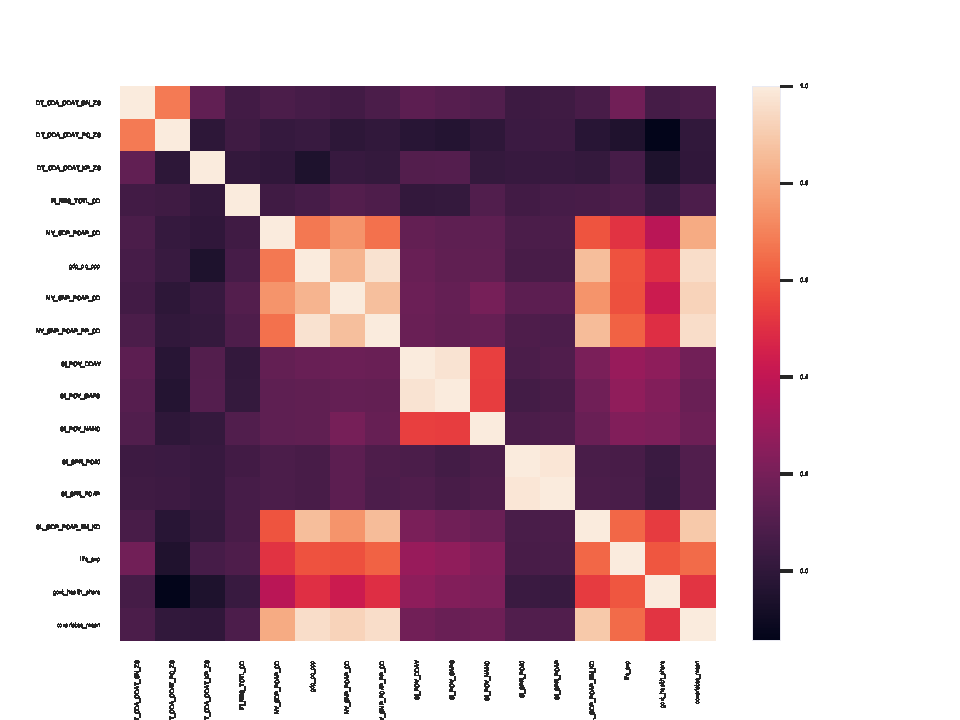
\includegraphics[width=\linewidth,keepaspectratio=true]{../Output/Figures/LE_Health_Econ_Correlations_wb_only_short.pdf}
        \end{figure}

        \begin{figure}[H]
            \centering
            \caption{Economic Measures PCA Loadings}
            \label{Econ_Loadings}	
            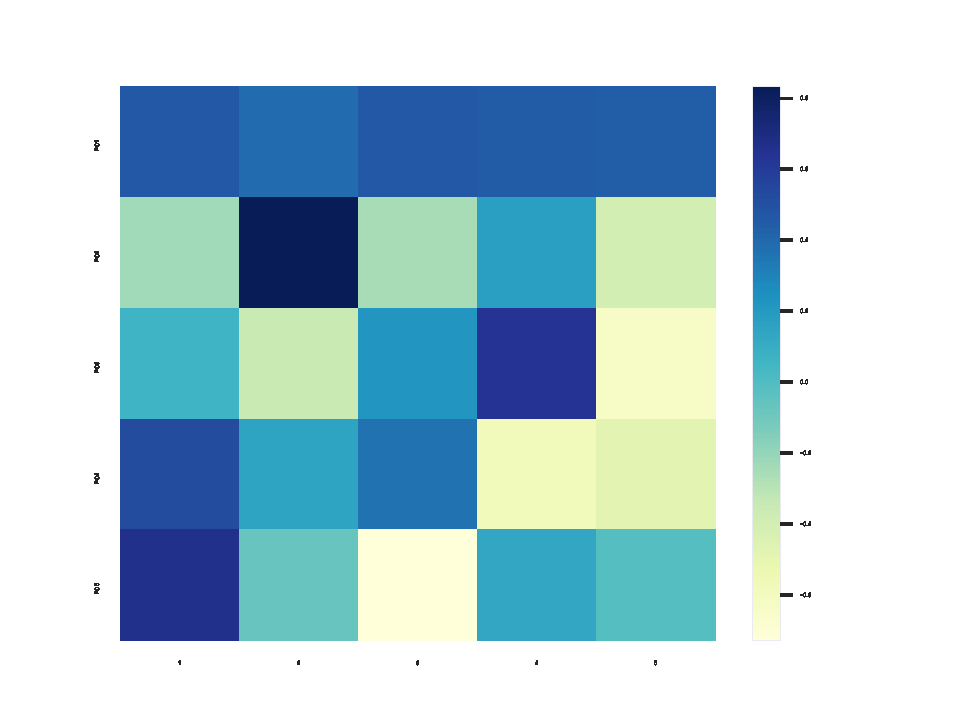
\includegraphics[width=\linewidth,keepaspectratio=true]{../Output/Figures/Econ_Indicator_Loadings_wb_only_short.pdf}
        \end{figure}

        \begin{figure}[H]
            \centering
            \caption{Economic Measures PCA Share of Variance Explained}
            \label{Econ_Share_Explained}	
            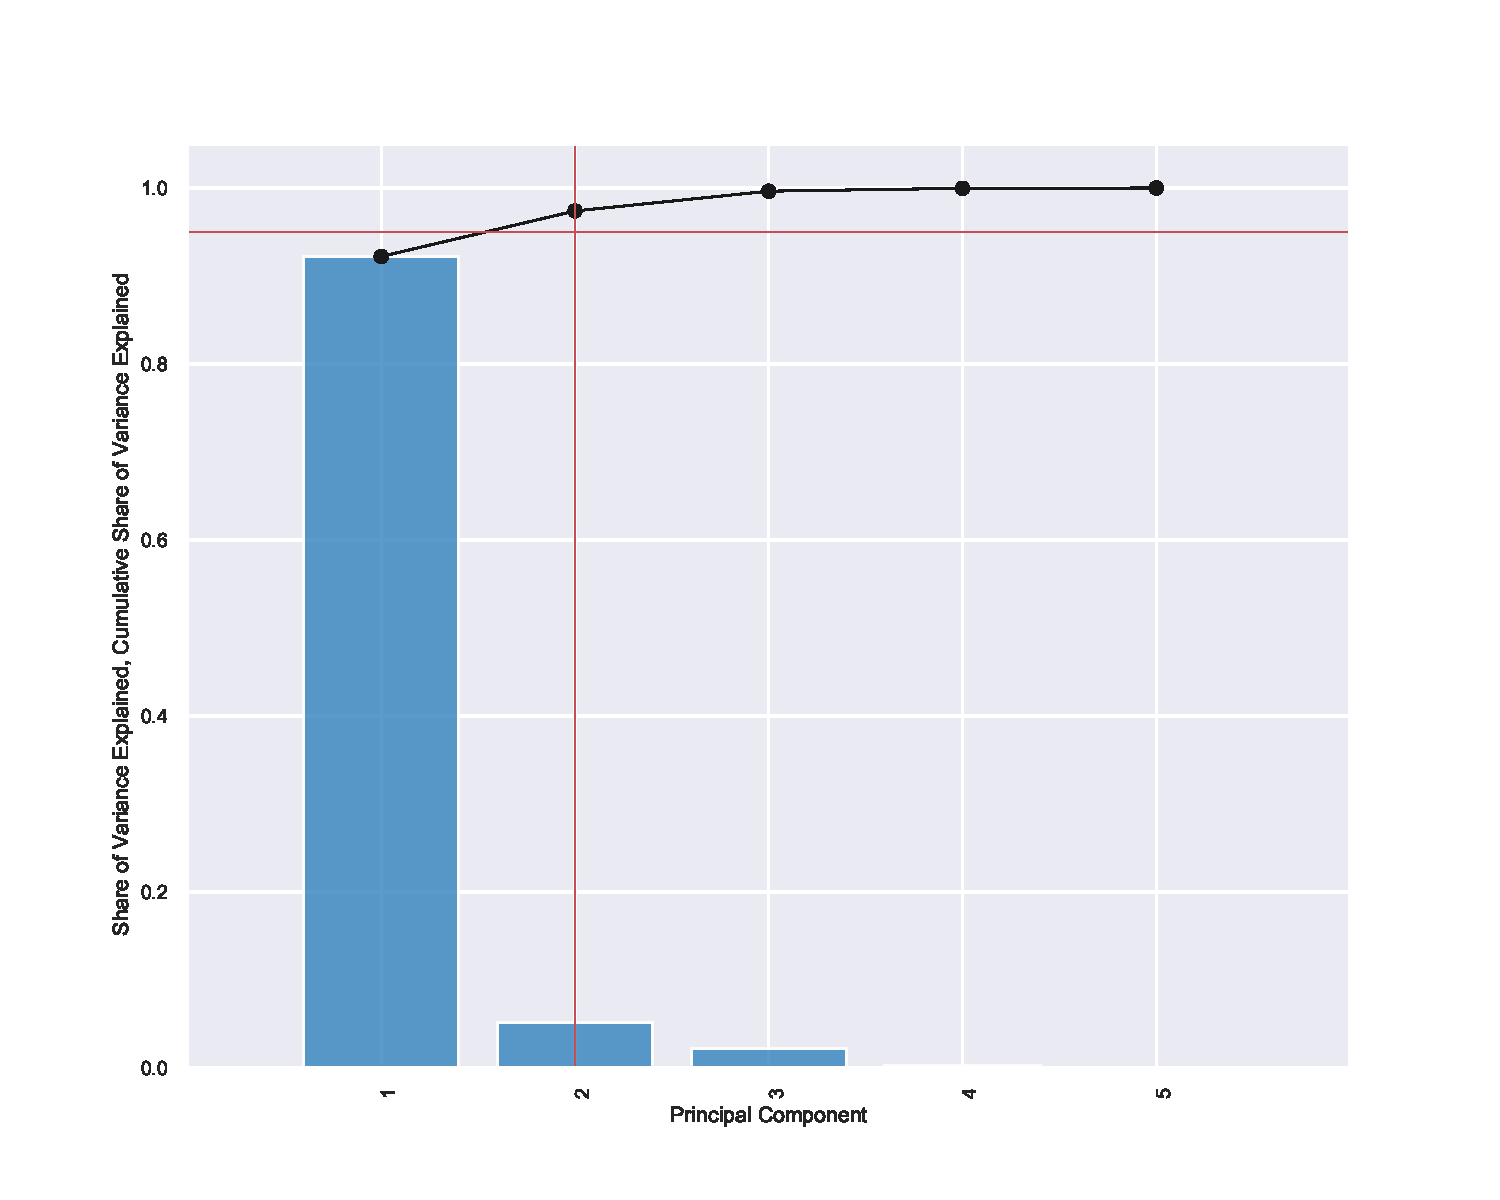
\includegraphics[width=\linewidth,keepaspectratio=true]{../Output/Figures/Econ_Indicator_Share_Explained_wb_only_short.pdf}
        \end{figure}

\end{document}